\section{UML Modellierung}

\begin{tcolorbox}[title=UML Modellierung]
    \textbf{Modelle} haben die Aufgabe, den Bezug zum Original (Programm, Softwaresystem) herzustellen, sowie zu der \textit{Anwendungsumgebung}.\\
    Ein \textbf{Modell} enthält alle \textbf{Modellelemente}, die zur Beschreibung eines Softwaresystems nötig sind.\\

    \noindent
    Ein \textbf{Modellelement} wird als Element in einem UML Modell von einem Benutzer erstellt und auf verschiedenen \textbf{Diagrammen} (Struktur-/Verhaltensdiagrammen) platziert, und wird durch die \textbf{UML Modellierungskonzepte} als Metaklasse des \textbf{Metamodells} der UML beschrieben: \textbf{Modellelemente} werden aus Modellierungskonzepten instanziiert.\\

    \noindent
       Das \textbf{UML Metamodell} regelt, in welchem Zusammenhang \textbf{UML Modellierungskonzepte} in Modellen auftreten dürfen, und welche Eigenschaften und Beziehungen zu anderen Sprachelementen zulässig sind.\\

       \noindent
       Die im \textbf{Metamodell} verwendeten Erklärungen basieren auf einer abstrakten Syntax, für deren Beschreibung eine Untermenge (\textit{Klassendiagramme}) der UML verwendet wird.\\
        Die \textbf{Semantik} der Modellierungskonzepte wird textlich beschrieben, zur Formalisierung von Regeln für die syntaktische Korrektheit wird die \textbf{OCL} (\textit{Object Constraint Language}) verwendet.
\end{tcolorbox}

\begin{figure}
    \centering
    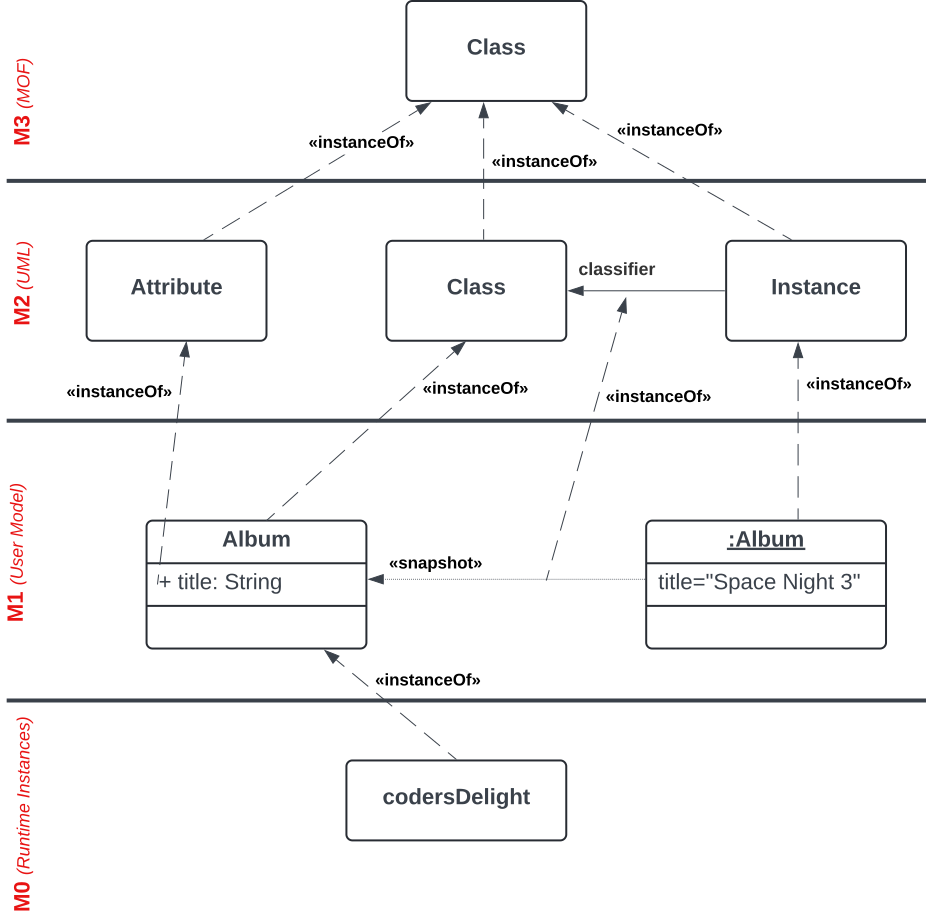
\includegraphics[scale=0.4]{part three/Einführung/img/metamodel}
    \caption{Beispiel für die verschiedenen Schichten der Metamodell Hierarchie.
        In der original Abbildung sind die Pfeilspitzen offen. (Quelle: in Anlehnung an S. 20, Figure 7.8, \url{https://www.omg.org/spec/UML/2.4.1/Infrastructure/PDF}, abgerufen 01.05.2024}
    \label{fig:metamodel-cc}
\end{figure}
